\documentclass[tikz,border=3mm]{standalone}
\usepackage{fontspec}
\usetikzlibrary{arrows.meta,calc,positioning,decorations.pathmorphing}
\definecolor{sulfur}{HTML}{E4B522}
\definecolor{sulfurdeep}{HTML}{A56C00}
\definecolor{polymer}{HTML}{34495E}
\definecolor{blue}{HTML}{2474A6}
\definecolor{cyan}{HTML}{68C3D4}
\definecolor{red}{HTML}{C84B31}
\definecolor{purple}{HTML}{7251A2}
\definecolor{green}{HTML}{3B8C6E}
\definecolor{ink}{HTML}{263238}
\definecolor{muted}{HTML}{66757F}
\definecolor{paper}{HTML}{F7F8F8}
\tikzset{
  >={Latex[length=2mm]},
  panel/.style={draw=ink!35,fill=white,rounded corners=2mm,line width=.55pt},
  label/.style={font=\sffamily\scriptsize,text=ink},
  small/.style={font=\sffamily\tiny,text=muted},
  title/.style={font=\sffamily\bfseries\small,text=ink},
  flow/.style={-{Latex[length=2mm]},line width=.8pt},
  sulfur atom/.style={circle,draw=sulfurdeep,fill=sulfur,minimum size=3.2mm,inner sep=0pt},
  charge/.style={circle,fill=red!85,text=white,font=\sffamily\bfseries\tiny,inner sep=1pt}
}
\newcommand{\panelhead}[2]{
  \draw[panel] (0,0) rectangle (5.8,4.9);
  \node[fill=ink,text=white,font=\sffamily\bfseries\small,
        rounded corners=1mm,minimum width=5mm,minimum height=5mm] at (.38,4.52) {#1};
  \node[title,anchor=west] at (.72,4.52) {#2};
  \draw[ink!18] (.2,4.18)--(5.6,4.18);
}
\begin{document}
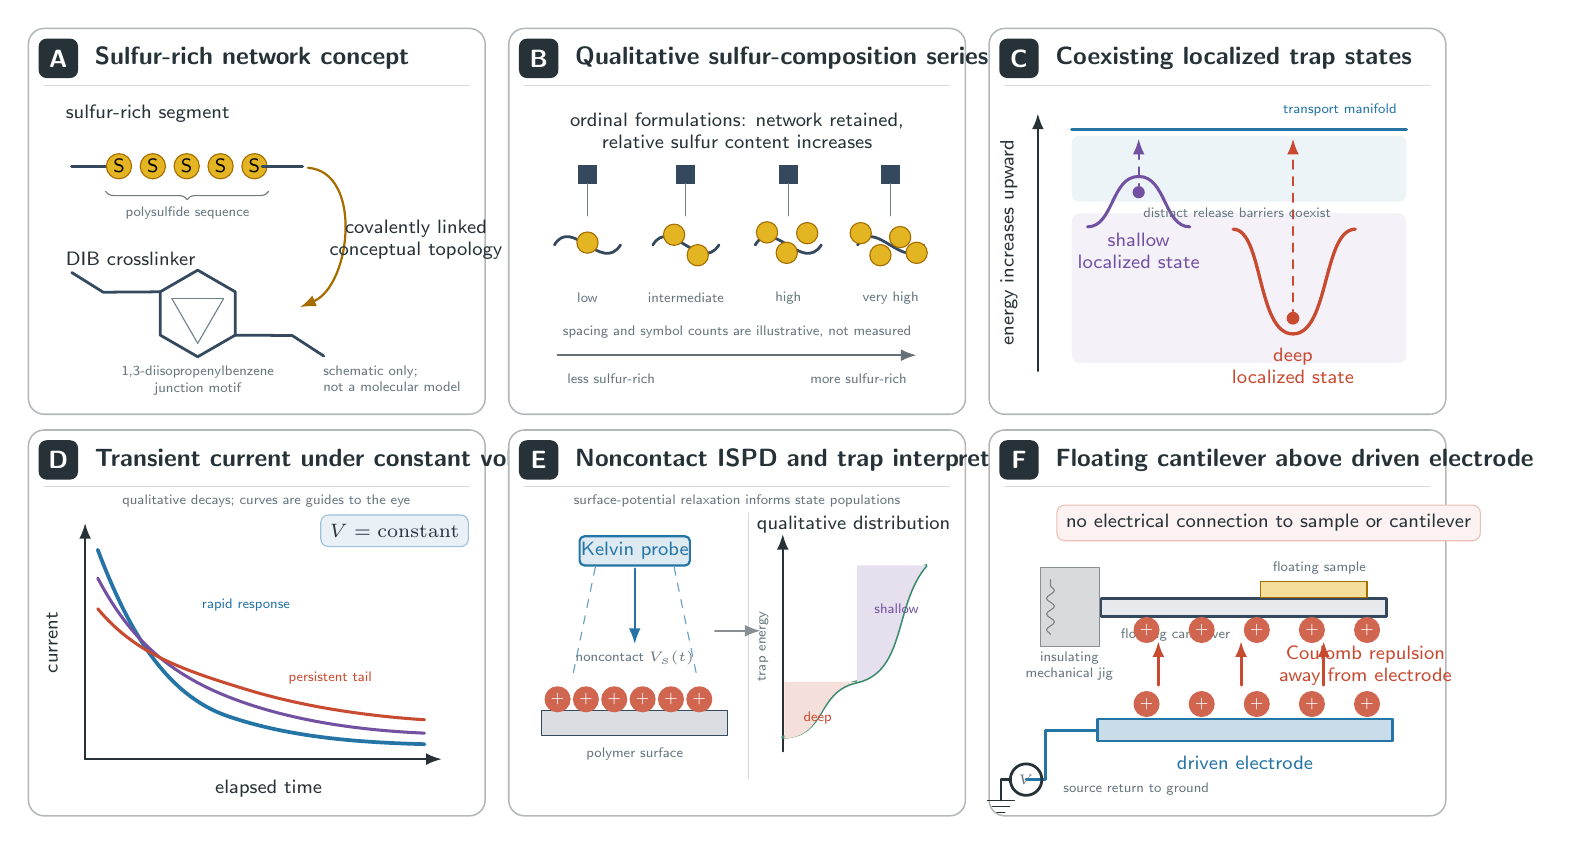
\begin{tikzpicture}[x=1cm,y=1cm,line cap=round,line join=round]
\sffamily

% A — conceptual network chemistry
\begin{scope}[shift={(0,5.1)}]
\panelhead{A}{Sulfur-rich network concept}
\node[label,anchor=west] at (.35,3.82) {sulfur-rich segment};
\draw[polymer,line width=1.2pt] (.55,3.15)--(1.05,3.15);
\foreach \x in {1.15,1.58,2.01,2.44,2.87}{
  \node[sulfur atom] at (\x,3.15) {\scriptsize S};
}
\draw[polymer,line width=1.2pt] (2.97,3.15)--(3.48,3.15);
\draw[decorate,decoration={brace,amplitude=3pt,mirror},ink!65]
  (.98,2.83)--(3.05,2.83);
\node[small] at (2.02,2.55) {polysulfide sequence};
\node[label,anchor=west] at (.35,1.98) {DIB crosslinker};
\coordinate (c) at (2.15,1.28);
\foreach \a in {30,90,...,330}{
  \coordinate (h\a) at ($(c)+(\a:0.55)$);
}
\draw[polymer,line width=1pt] (h30)--(h90)--(h150)--(h210)--(h270)--(h330)--cycle;
\draw[polymer!70] ($(c)+(30:.38)$)--($(c)+(150:.38)$);
\draw[polymer!70] ($(c)+(150:.38)$)--($(c)+(270:.38)$);
\draw[polymer!70] ($(c)+(270:.38)$)--($(c)+(30:.38)$);
\draw[polymer,line width=1pt] (h150)--(.95,1.55)--(.55,1.80);
\draw[polymer,line width=1pt] (h330)--(3.35,1.00)--(3.75,.74);
\node[small,align=center] at (2.15,.43) {1,3-diisopropenylbenzene\\junction motif};
\draw[flow,sulfurdeep] (3.55,3.13) .. controls (4.25,3.08) and (4.10,1.64) .. (3.45,1.36);
\node[label,align=center,anchor=west] at (3.70,2.22) {covalently linked\\conceptual topology};
\node[small,align=left,anchor=west] at (3.62,.45) {schematic only;\\not a molecular model};
\end{scope}

% B — ordinal composition series
\begin{scope}[shift={(6.1,5.1)}]
\panelhead{B}{Qualitative sulfur-composition series}
\draw[flow,ink!70] (.62,.75)--(5.18,.75);
\node[small,anchor=west] at (.62,.45) {less sulfur-rich};
\node[small,anchor=east] at (5.18,.45) {more sulfur-rich};
\foreach \x/\n/\lab in {1.0/1/low,2.25/2/intermediate,3.55/3/high,4.85/4/very high}{
  \draw[polymer,line width=1pt] (\x-.42,2.15) .. controls (\x-.2,2.52) and (\x+.18,1.78) .. (\x+.42,2.15);
  \node[small] at (\x,1.48) {\lab};
}
\foreach \p in {(1.00,2.18),(2.10,2.28),(2.40,2.02),(3.28,2.31),(3.53,2.05),(3.79,2.30),(4.47,2.30),(4.72,2.02),(4.97,2.25),(5.18,2.05)}
  \node[sulfur atom,minimum size=2.7mm] at \p {};
\foreach \x in {1.0,2.25,3.55,4.85}{
  \node[rectangle,fill=polymer,minimum width=2.4mm,minimum height=2.4mm,inner sep=0pt] at (\x,3.05) {};
  \draw[polymer!70] (\x,2.93)--(\x,2.52);
}
\node[label,align=center] at (2.9,3.60) {ordinal formulations: network retained,\\relative sulfur content increases};
\node[small,align=center] at (2.9,1.05) {spacing and symbol counts are illustrative, not measured};
\end{scope}

% C — hero trap landscape
\begin{scope}[shift={(12.2,5.1)}]
\panelhead{C}{Coexisting localized trap states}
\draw[flow,ink] (.62,.55)--(.62,3.82);
\node[label,rotate=90] at (.25,2.18) {energy increases upward};
\draw[blue,line width=1.2pt] (1.05,3.62)--(5.30,3.62);
\node[small,anchor=east,text=blue] at (5.30,3.86) {transport manifold};
\fill[blue!8,rounded corners=1mm] (1.05,2.70) rectangle (5.30,3.54);
\fill[purple!8,rounded corners=1mm] (1.05,.65) rectangle (5.30,2.55);
\draw[purple,line width=1.1pt]
  (1.25,2.38) .. controls (1.58,2.38) and (1.55,3.02) .. (1.90,3.02)
  .. controls (2.25,3.02) and (2.22,2.38) .. (2.55,2.38);
\fill[purple] (1.90,2.82) circle (2.2pt);
\draw[red,line width=1.2pt]
  (3.10,2.35) .. controls (3.48,2.35) and (3.40,1.02) .. (3.86,1.02)
  .. controls (4.32,1.02) and (4.24,2.35) .. (4.65,2.35);
\fill[red] (3.86,1.22) circle (2.3pt);
\draw[flow,dashed,purple] (1.90,2.82)--(1.90,3.50);
\draw[flow,dashed,red] (3.86,1.22)--(3.86,3.50);
\node[label,text=purple,align=center] at (1.90,2.08) {shallow\\localized state};
\node[label,text=red,align=center] at (3.86,.62) {deep\\localized state};
\node[small,align=center] at (3.15,2.56) {distinct release barriers coexist};
\end{scope}

% D — qualitative current transient
\begin{scope}[shift={(0,0)}]
\panelhead{D}{Transient current under constant voltage}
\draw[flow,ink] (.72,.72)--(.72,3.72);
\draw[flow,ink] (.72,.72)--(5.25,.72);
\node[label,rotate=90] at (.30,2.20) {current};
\node[label] at (3.05,.35) {elapsed time};
\node[label,fill=blue!10,draw=blue!45,rounded corners=1mm] at (4.65,3.62) {$V=\mathrm{constant}$};
\draw[blue,line width=1.35pt]
  (.88,3.38) .. controls (1.25,2.40) and (1.72,1.55) .. (2.52,1.27)
  .. controls (3.35,.98) and (4.30,.93) .. (5.03,.91);
\draw[purple,line width=1.1pt]
  (.88,3.02) .. controls (1.30,2.22) and (1.82,1.78) .. (2.62,1.48)
  .. controls (3.45,1.17) and (4.36,1.08) .. (5.03,1.05);
\draw[red,line width=1.1pt]
  (.88,2.63) .. controls (1.34,2.08) and (1.90,1.87) .. (2.72,1.62)
  .. controls (3.55,1.36) and (4.42,1.26) .. (5.03,1.22);
\node[small,text=blue,anchor=west] at (2.08,2.68) {rapid response};
\node[small,text=red,anchor=west] at (3.18,1.75) {persistent tail};
\node[small,align=center] at (3.02,4.00) {qualitative decays; curves are guides to the eye};
\end{scope}

% E — ISPD measurement and interpretation
\begin{scope}[shift={(6.1,0)}]
\panelhead{E}{Noncontact ISPD and trap interpretation}
\fill[polymer!18,draw=polymer] (.42,1.02) rectangle (2.78,1.34);
\node[small] at (1.60,.78) {polymer surface};
\foreach \x in {.62,.98,1.34,1.70,2.06,2.42}
  \node[charge] at (\x,1.48) {$+$};
\draw[fill=blue!15,draw=blue,line width=.8pt,rounded corners=.6mm] (.90,3.18) rectangle (2.30,3.55);
\node[label,text=blue] at (1.60,3.37) {Kelvin probe};
\draw[dashed,blue!70] (1.10,3.16)--(.80,1.72);
\draw[dashed,blue!70] (2.10,3.16)--(2.40,1.72);
\draw[flow,blue] (1.60,3.14)--(1.60,2.18);
\node[small,align=center] at (1.60,2.00) {noncontact $V_s(t)$};
\draw[ink!20] (3.05,.48)--(3.05,3.85);
\draw[flow,ink] (3.48,.82)--(3.48,3.58);
\node[small,rotate=90] at (3.23,2.15) {trap energy};
\draw[green,line width=1.2pt]
  (3.48,1.00) .. controls (4.05,1.02) and (3.88,1.58) .. (4.42,1.70)
  .. controls (5.04,1.84) and (4.88,2.70) .. (5.30,3.18);
\fill[red!18] (3.50,.98) .. controls (4.05,1.02) and (3.88,1.58) .. (4.42,1.70)
  --(3.50,1.70)--cycle;
\fill[purple!18] (4.42,1.70) .. controls (5.04,1.84) and (4.88,2.70) .. (5.30,3.18)
  --(4.42,3.18)--cycle;
\node[small,text=red,anchor=west] at (3.62,1.24) {deep};
\node[small,text=purple,anchor=west] at (4.52,2.63) {shallow};
\node[label,align=center] at (4.38,3.70) {qualitative distribution};
\draw[flow,ink!55] (2.62,2.35)--(3.20,2.35);
\node[small,align=center] at (2.90,4.00) {surface-potential relaxation informs state populations};
\end{scope}

% F — floating cantilever and driven electrode
\begin{scope}[shift={(12.2,0)}]
\panelhead{F}{Floating cantilever above driven electrode}
\fill[polymer!12,draw=polymer,line width=1pt] (1.42,2.53) rectangle (5.05,2.76);
\fill[sulfur!45,draw=sulfurdeep] (3.45,2.77) rectangle (4.80,2.98);
\node[small,anchor=west] at (3.48,3.15) {floating sample};
\fill[ink!18,draw=ink!55] (.65,2.15) rectangle (1.40,3.15);
\draw[decorate,decoration={snake,amplitude=.5mm,segment length=2mm},ink!60]
  (.78,2.30)--(.78,3.00);
\node[small,align=center] at (1.02,1.90) {insulating\\mechanical jig};
\node[small,anchor=west] at (1.55,2.30) {floating cantilever};
\fill[blue!25,draw=blue,line width=1pt] (1.38,.95) rectangle (5.12,1.23);
\node[label,text=blue] at (3.25,.68) {driven electrode};
\foreach \x in {2.0,2.7,3.4,4.1,4.8}{
  \node[charge] at (\x,1.42) {$+$};
  \node[charge] at (\x,2.36) {$+$};
}
\foreach \x in {2.15,3.20,4.25}
  \draw[flow,red,line width=1.05pt] (\x,1.66)--(\x,2.22);
\node[label,text=red,align=center] at (4.78,1.91) {Coulomb repulsion\\away from electrode};
\draw[blue,line width=1pt] (1.38,1.08)--(.72,1.08)--(.72,.46)--(.47,.46);
\draw[ink,line width=1pt] (.47,.46) circle (.20);
\node[small] at (.47,.46) {$V$};
\draw[ink,line width=1pt] (.27,.46)--(.15,.46)--(.15,.20);
\draw[ink] (-.02,.20)--(.32,.20) (.04,.12)--(.26,.12) (.10,.04)--(.20,.04);
\node[small,anchor=west] at (.82,.34) {source return to ground};
\node[label,fill=red!7,draw=red!35,rounded corners=1mm,align=center] at (3.55,3.72)
  {no electrical connection to sample or cantilever};
\end{scope}

\end{tikzpicture}
\end{document}
